% Use only LaTeX2e, calling the article.cls class and 12-point type.

\documentclass[12pt]{article}

% Users of the {thebibliography} environment or BibTeX should use the
% scicite.sty package, downloadable from *Science* at
% www.sciencemag.org/about/authors/prep/TeX_help/ .
% This package should properly format in-text
% reference calls and reference-list numbers.

\usepackage{scicite}

% Use times if you have the font installed; otherwise, comment out the
% following line.

\usepackage{times}
\usepackage{amsmath}
\usepackage{amssymb}
\usepackage{graphicx}
\usepackage{subcaption}
\graphicspath{ {./images/} }

% The preamble here sets up a lot of new/revised commands and
% environments.  It's annoying, but please do *not* try to strip these
% out into a separate .sty file (which could lead to the loss of some
% information when we convert the file to other formats).  Instead, keep
% them in the preamble of your main LaTeX source file.


% The following parameters seem to provide a reasonable page setup.

\topmargin 0.0cm
\oddsidemargin 0.2cm
\textwidth 16cm 
\textheight 21cm
\footskip 1.0cm


%The next command sets up an environment for the abstract to your paper.

\newenvironment{sciabstract}{%
\begin{quote} \bf}
{\end{quote}}


% If your reference list includes text notes as well as references,
% include the following line; otherwise, comment it out.


% The following lines set up an environment for the last note in the
% reference list, which commonly includes acknowledgments of funding,
% help, etc.  It's intended for users of BibTeX or the {thebibliography}
% environment.  Users who are hand-coding their references at the end
% using a list environment such as {enumerate} can simply add another
% item at the end, and it will be numbered automatically.

\newcounter{lastnote}
\newenvironment{scilastnote}{%
\setcounter{lastnote}{\value{enumiv}}%
\addtocounter{lastnote}{+1}%
\begin{list}%
{\arabic{lastnote}.}
{\setlength{\leftmargin}{.22in}}
{\setlength{\labelsep}{.5em}}}
{\end{list}}
\newcommand{\vect}[1]{\boldsymbol{#1}}


\title{{\it Using a convolutional neural network to classify the Street View House Number dataset}}

\author
{Andrea Ferretti\\
\normalsize{andrea.ferretti1@studenti.unimi.it}
}

% Include the date command, but leave its argument blank.

\date{}


\begin{document} 

% Double-space the manuscript.

\baselineskip24pt

% Make the title.

\maketitle 

\begin{sciabstract}

This report serves as a descriprion of 

\end{sciabstract}

\section*{Neural networks}
Neural networks are a family of predictors characterized by the combination of simple computational units, called neurons.
A neuron typically performs the following computation: $ g(\vect{x}) = \sigma(\vect{\omega}^T \vect{x}) $, where the elements of the vector $\vect{\omega}$ are the parameters of the neuron, $\sigma$ is a non-linear function called activation function, and $\vect{x}$ is the vector $x_0,\ldots,x_n $ where $ x_0 = 1$ and $x_i$ for $i \in \{i,\ldots,n\}$  the output computed by another neuron.
In the supervised learning setting, neurons are combined in a graph-like structure resulting in a computational network able to learn, by adjusting the parameters $\vect{\omega}$ of each neuron, the underlying mapping between data points and their corresponding labels.

One of the most basic architecture a neural network can assume is called feedforward network. In this type of network neurons are organized into successive layers: one input layer, one or more hidden layers, and one output layer. The computation flows from the input layer towards the output layer and each neuron passes its output to all the neurons in the next layer. The $i$-th neuron in the input layer simply outputs the value of the $i$-th dimension of the data point. The neurons in the other layers compute a non-linear function of the weighted sum of the outputs of the neurons in the previous layer (plus a bias), every neuron has therefore his own vector of weights and a bias term. The funciton computed by the neurons in the hidden layers is called the activation function and usually is some kind of sigmoid function such as the logistic function:
\begin{equation}
\label{eq:sigmoid}
S(x) = \frac{1}{1 + e^{-x}}
\end{equation}\\
The neurons in the output layer compute a function that varies depending on the type of problem: for a regressor the identity function can be used to obtain a real valued output for each neuron, for a classifier, instead, the softmax function is typically used. The softmax function $ softmax: \mathbb{R}^m \rightarrow \mathbb{R}^m $ is defined as:
\begin{equation}
\label{eq:softmax}
softmax(\vect{v})_i = \frac{e^{\vect{v}_i}}{\sum_{t=0}^{m}e^{\vect{v}_t}} \text{, for } i = 0,\ldots,m-1 \text{ and } \vect{v} \in \mathbb{R}^m
\end{equation}
By having a network with as many output neurons as the number of possible classes to be predicted a probability distribution over those classes is obtained using softmax. It is to note that, in order for this function to be computed, every output neuron needs to know the values of the other output neurons (the various $ \vect{v}_t$) before the softmax is applied. Figure \ref{fig:mlp} gives an example of a feedforward neural network.

\begin{figure}[h]
	\centering
	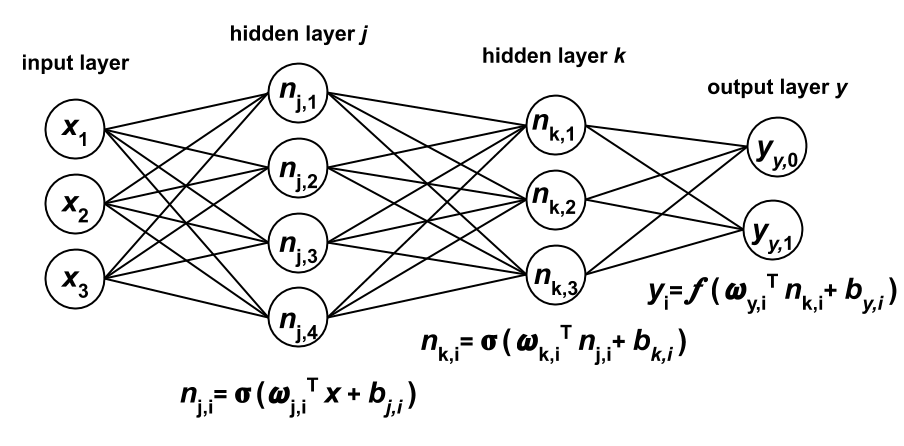
\includegraphics[width=\textwidth]{mlp}
	\caption{A feedforward network where on each neuron there is a label representing the value computed by it and passed to the nodes of the next layer through the arcs connecting them. A neuron assigns a weight $ \omega $ to each incoming arch and performs the shown linear combination. The sigmoid funciton of equation (\ref{eq:sigmoid}) can be used as the activation function $\sigma$. The function computed by the neurons in the output layer could be $softmax$ (\ref{eq:softmax}) where $\vect{v}_i = \vect{\omega}_{y,i}^T\vect{n}_k + b_{y,i}$. Here the bias $ b $ is explicited in the computation rather than adding another dimension to the various vectors $ \vect{\omega} $, $ \vect{n}$, and $ \vect{x} $ so that $ \omega_{r,i,0} = b_{r,i} $ for $ r \in \{j,k,y\} $ and $ x_{0} = n_{p,0} = 1 $ for $p \in \{j,k\} $.}
\label{fig:mlp}
\end{figure}

Consider the pair $(\vect{x}, y)$ consisting of a data point and its corresponding label, let $\vect{\hat{{y}}}$ be the output of the network, in order to assest the goodness of the prediction a non-negative loss function $\ell(y,\vect{\hat{y}})$ is used so that the greater its value the worse is the prediciton. In the case of a classification problem $y \in Y$, where $Y$ is the ordered set of possible symbolic labels with $|Y| = m$, therefore, by having a network with $m$ neurons in the output layer and using the $softmax$ function, the network prediction $\vect{\hat{y}}$ represents a probability distribution over $Y$ given the data point $\vect{x}$. For conveniency of notation let $y^*_i$ indicate the first element of $Y$ for $i = 0$, the second element of $Y$ for $i = 1$ and so on for all the elements of $Y$. This means that the $i$-th element of $\vect{\hat{y}}$ gives the probability that the label for the data point $\vect{x}$ will be $y^*_i$ in the network prediction. In this case, as loss function, the categorical cross-entropy loss can be used and it is defined as:
\begin{equation}
\label{eq:cross-entropy}
\ell(y,\vect{\hat{y}}) = -\sum_{i=0}^{m-1}{P(y = y^*_i)\log(\hat{y_i})} 
\end{equation}
where $P(y = y^*_i)$ is the probability that the true label for the data point $\vect{x}$ is $y^*_i$. Since , in practice, to a single data point in the training set corresponds only one label with probability $1$, 
equation (\ref{eq:cross-entropy}) can be simplified to:
$$
\ell(y,\vect{\hat{y}}) = -\sum_{i=0}^{m-1}{\mathbb{I}(y = y^*_i)\log(\hat{y_i})}  = -log(\hat{y_i}) \text{, where } i \text{ verifies } y^*_i = y
$$
where $\mathbb{I}(E) \in \{0, 1\}$ is the indicator function of an event $E$, meaning that $\mathbb{I}(E) = 1$ if and only if $E$ occours and $\mathbb{I}(E) = 0$ otherwise.

Given the loss function $\ell$ the network can be trained on the training data to minimize $\ell$ with respect to the parameters of each neuron. This is typically done with the mini-batched stochastic gradient descent algorithm, where, at each timestep, a fixed number of examples creating a subset $B^{(t)}$ of the training set is randomly selected and every parameter is iteratively updated following the rule:
\begin{equation}
\label{eq:sgd}
\omega_{l,n,i}^{(t+1)} \leftarrow \omega_{l,n,i}^{(t)} - \eta^{(t)}\frac{1}{|B^{(t)}|}\sum_{b \in B^{(t)}}{\frac{\partial \ell^{(t)}(y_b,\vect{\hat{y}}_b)}{\partial \omega_{l,n,i}}}
\end{equation}
where, as depicted in Figure \ref{fig:mlp}, $\omega_{l,n,i}$ represents the $i$-th parameter of the $n$-th neuron in the $l$-th layer, and $\vect{\hat{y}}_b$ is the output computed by the network for the example $(x_b, y_b)$ of the training set; $\eta_t$ is the learning rate that determines the update size. To calculate efficiently the partial derivatives with respect to all the parameters $\omega$ the backpropagation algorithm is used. The algorithm uses the chain rule to compute the derivative of a composite function:
$$
\frac{df(g(x))}{dx} = \frac{df(g)}{dg} \frac{dg(x)}{dx}
$$
When using a sigomid as the activation function of the neurons, the networks can experience the so called vanishing gradient problem, in which the gradients of the sigmoids of several neurons become so small that the several multiplications of the chain rule cause, especially in deep networks, the update of the weight depending on those gradients to be almost non existant. This happens because the sigmoid function has small gradients for high absolute value inputs; one possible solutoin is to use the rectifier $f(x) = max(0,x)$ as the activation function, this allows the gradient to always be equal to 1 when the output of the neuron is non-negative.

For input data that presents a grid-like structure a specific kind of network architecture called convolutional neural network (abbreviated ConvNet) has been developed. Similarly to feedforward networks it retains the forward direction of the computation, but it adds different types of layers such as convolutional layers and pooling layers. A convolutional layer is composed of several filters (also called kernels), each one performs a spatial convolution applying itself over the input dimensions; the output volume produced by this layer is called a feature map.
A filter is composed by a mutlidimensional vector where each element is a real number called weight, and a single bias. Applying a filter over a portion of the input volume consist in multiplying each element of the input with the corresponding  weight, then all the products are added together, along with the bias term, and the sum is used as input to the non-linear activation function producing the final single-valued result. The filter is then slid along the dimenions of the input and the operations are repeated to form one channel of the feature map; stacking together the results of convolutions of multiple filters the complete feature map is obtained. Considering as an example the case of creating a convolutional layer for a RGB image, the input (the image) can be seen as a 2 dimensional volume with 3 channels. The filter will therefore be 3 dimensional and slide along the 2 dimensions of the input, and the result of convoluting the filter will be a 2 dimensional output. The size of the first 2 dimensions of the filter, who both affect how big the portion of the input captured by one applicaton is, can be chosen freely, but the third dimension needs to be the equal to the number of channels of the input, otherwise applying the filter would not be possible. In order for the sizes of the output dimensions to be equal to the input ones the input can be padded with zero valued elements. Adding more equally dimensioned filters to the layer increases the number of channels the output volume will have. The parameters of a convolutional layer are therefore given by the weights and biases of each filter. During training the network can learn which parameters allow filters to extract the most relevant features from the input.\\
The pooling layer function is to reduce the spatial size of a feature map, practically downsampling the convolutional layer output in order to decrease the total number of parameters and the computational burden of the network. It does so using a particular kind of filter, that returns the maximum value among the ones it's being applied on, sliding it across the dimensions of each input channel indipendently. The output produced has the same number of channels as the input but the size of the other dimensions is reduces. This way only the most dominant features detected by the convolutional layer are retained. Going back to the RGB image example, assuming that a convolutional layer used 10 filters and produced a feature map where the first and second dimensions are equal to 30, a pooling layer, whose filter is of size 2 on both dimension and slides across with a stride of 2 elements, outputs a volume of size 15 on both dimension and 10 channels.\\
A typical ConvNet combines a variable number of blocks composed of one or more convolutional layer followed by a pooling layer (it is to note that if the sizes of the feature map produced by the convolutional layer are already small, the pooling layer may be avoided). The last output volume of this chain is then flattened into a one dimensional vector, losing its grid-like structure, and connected to a feedforward network that handles the classification part. This allows to have the same loss function as a feedforward network and to similarly train the weights via stochastic gradient descent. Figure \ref{fig:cnn} shows one of the possible structures of a ConvNet. 

\begin{figure}[h]
	\centering
	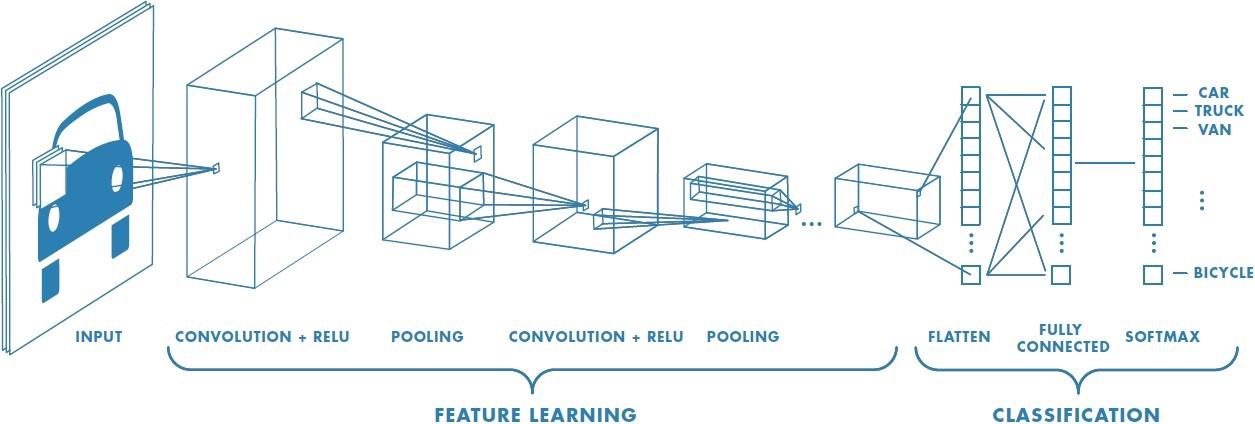
\includegraphics[width=\textwidth]{cnn}
	\caption{A visual representation of a convolutional neural network applied to image classification. The main components are: the convolutional layers producing the feature maps, the pooling layers used to downsample the convolutional layers output, and a standard fully connected feedforward network to handle classification}
	\label{fig:cnn}
\end{figure}

Regularization consists in setting costraints to the model in order to avoid overfitting of the training set. Several techniques have been developed: L2 regularization adds to the loss function a fraction of the L2 norm of the weights, penalizing models where some of the weights have a value much greater that the rest; this is done to increase the generalization capabilities by incouraging the model to use all the input values when making a prediciton, instead of having few input dimensions heavily influencing the prediction.
Dropout	consists in randomly (with a fixed probability) dropping neurons, along with their connections, from the network during training, preventing neurons from co-adapting too much. At test time all neurons are active and their outputs are scaled to match the output during training in expectation.

Lastly batch normalization is seen as a normalization technique that normalizes the output of each neuron with respect to the values produced by that neuron for the batch that the network it's iterating over during training, the normalized value is then linearly transormed to give the data a new distribution. The parameters that determine this transofrmation are learnt throught training. Batch normalization has been shown to improve the prediction performance even though the interpretation of its operation is not yet completely clear.


\section*{The dataset}
The Street View House Number dataset consists of real world RGB images obtained from house numbers in Google Street View. The images are available in two format: the original, variable-resolution, images, with a separate file describing the position of each digit in the image (shown in Figure \ref{fig:svhn1}), and
32 by 32 pixels images centered around a single digit, an example of the second format is shown in Figure \ref{fig:svhn2}.

\begin{figure}[h]\centering
	\begin{subfigure}{\textwidth}
		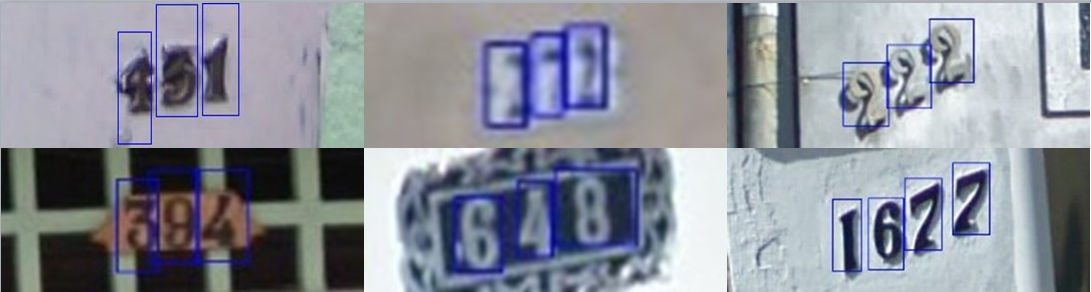
\includegraphics[width=\textwidth]{svhn-ocr}
		\caption{The first format}
		\label{fig:svhn1}
	\end{subfigure}

	\begin{subfigure}{\textwidth}
		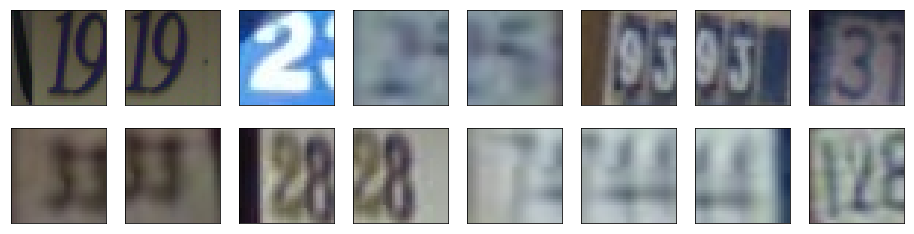
\includegraphics[width=\textwidth]{svhn-centered}
		\caption{The second format}
		\label{fig:svhn2}
	\end{subfigure}
	\label{fig:svhn}
	\caption{(a) The original images obtained from Street View. The blue rectangles describe the position of each digit in the images, they are shown for clarity but are not present in the images, their coordinates are stored in a separate file. (b) The images cropped and centered around a single digit. Note the presence of other digits to the sides of the one centered}
\end{figure}

The second format, with the images already cropped and centered around the digit to predict, is certanly to prefer for a classification problem. This is due to the fact that the input are all of the same shape and the format is similar to other datasets that have been extensively analyzed. It is to note that the preprocessing done leaves nonetheless other digits in the image that are nonrelevant to the prediction, from this a greater degree of difficulty than just predicting a single isolated digit arises.
The faced problem is therefore a classification problem where the input are 32 by 32 pixels images classified into 10 classes, where an image representing a 9 has a numerical label 9, 1 has a numericla label 1 and so on, except for 0 which has label 10 in the dataset. The training set contains 73257 images and the test set 26032. Additional 531131, somewhat less difficult, images are available to use as extra training images, but they will not be used in this experiment. A validation set for hyperparameter tuning has been randomly extraced from the training set, the validation set size is 10\% of the original training set size; this resulted in a smaller training set during the model design phase.
The distribution of the labels for the data sets is shown in Figure \ref{fig:hist}. Because of the nature of house numbering it is expected to see a higher presence of lower digits, particulary 1 and 2.

\begin{figure}[h]
	\centering
	\begin{subfigure}{0.31\textwidth}
		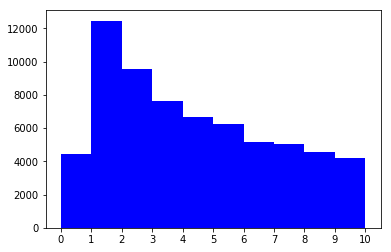
\includegraphics[width=\linewidth]{hist_train}
		\caption{Training set}
		\label{fig:hista}
	\end{subfigure}
	\hspace*{\fill} % separation between the subfigures
	\begin{subfigure}{0.31\textwidth}
		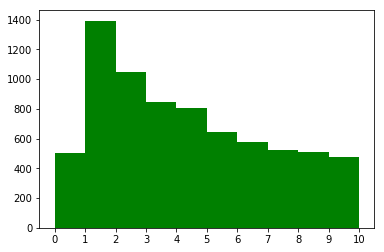
\includegraphics[width=\linewidth]{hist_validation}
		\caption{Validation set}
		\label{fig:histb}
	\end{subfigure}
	\hspace*{\fill} % separation between the subfigures
	\begin{subfigure}{0.31\textwidth}
		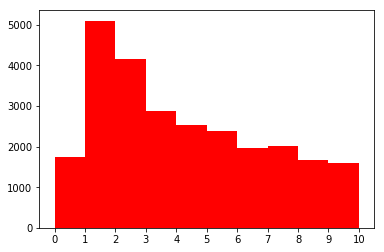
\includegraphics[width=\linewidth]{hist_test}
		\caption{Test set}
		\label{fig:histc}
	\end{subfigure}
	\caption{Histograms representing the absolute frequency of the labels for the training set (a), validation set (b), and test set (c). The distribution is very similar among the various sets, making it sound to use them for machine learning tasks.}
	\label{fig:hist}
\end{figure}
The data set can be obtained at the following website: http://ufldl.stanford.edu/housenumbers/

\section*{Model training}

The first step involved some data preprocessing. The images are colored but the colors do not seem to convey any usefull information that can be used to distinguish one digit from another, therefore the images have been converted form RGB to grayscale using the formula $ gv = 2989*r+0.5870*g+0.1140*b $ where $r, g, b$ are the pixel values for the red, green, and blue channels and $gv$ is the corresponding grayscale value of that pixel. This was followed by a mean subtraction and a normalization. Mean subtraction consists in subtracting the mean across every feature of the input, making them zero centered; for images, in particular, the mean among all the pixel in the training set can be calculated and subtracted instead. The normalization is obtained by dividing each pixel by the standard deviation of all the pixel after they have been zero centered. It is important to notice that the mean and the standard deviation have to be calculated on the training set only and then used to preprocess the training set, the validation set, and the test set. This is due to the fact that, in a real world scenario, the model can't have those statistics for future, never seen before, data points it will have to classify, and since the test set is supposed to approximate  those data points its statistics cannot be used.

In order to design the model and tune hyperparameters it has been used a form of cross validation consisting of the following steps: select a hyperparameter to optimize, traing the model for different values of that hyperparameter on the reduced training set (the reduced training set consists of the original training set from which examples added to the validation set have been removed), the model with the smallest loss on the validation set determines the value of the hyperparameter to choose; this process is then repeated for all the remaining non-optimized hyperparameters. It is worth noting that this does not represent a proper hyperparameter search since, once the value of a hyperparameter is chosen, the optimization of the remaining hyperparameters depends on the previously selected ones. A more correct way to perform the search, albeit much more computationally expensive, would be to train the model with numerous combinations of values of the hyperparameters and choosing the combination of values that performs best on the validation set; this method has not been performed in this experiment due to its computational burden.

As described in the first section of this report a ConvNet has typically three components: convolutional layers, pooling layers and a feedforward component. The base network architecture that has been proven to have good results for similar tasks consists of blocks made of one or more convolutional layers followed by  a pooling layer, these blocks are concatenated untill the output of the last pooling layer has a small enough size. At this point one or more convolutional layers can follow to increase the representational power of the network. The resulting output is then flattened into a vector and fed to a feedforward network with a softmax output layer for classification purpose. The filter of the convolutional layers have size equal to 3 on each dimension, these small filters have been shown to consistently perform better that larger filters, especially when stacking multiple convolutional layers on top of each other. The input of convolutional layers is zero-padded before performing the convolution so that the sizes of the output dimensions remain unchanged. The filters of the pooling layers have size equal to 2 for each dimension, halving the size of the input dimensions, otherwise larger filters would discard too much information. Considering the original input size is 32 by 32, no more than two pooling layers can be applied, otherwise the output would be smaller than 8 by 8 which would be too small to convey enough information for classification.

In the first section it was stated that parameters of the network can be updated using stochastic gradeint descent which follows the update rule (\ref{eq:sgd}) where the learning rate $\eta^{(t)}$ at timestemp $t$ is a hyperparameter. Adam, short for Adaptive Moment Estimation, is used in this experiment instead; it is a more recent technique that improves convergence time and adjusts the learning rate for each parameter based on the update rule:
$$
\vect{\omega}^{(t+1)}\leftarrow \vect{\omega}^{(t)}-\eta^{(t)} {\frac {\vect{{\hat {m}}}_{\omega}}{{\sqrt {\vect{{\hat {v}}}_{\omega}}}+\epsilon }}
$$
where $\vect{\omega}^{(t)}$ is the vector of parameters at time step $t$, $\epsilon$ is a small constant to avoid division by zero, and	 $\vect{{\hat {m}}}_{\omega}$ and $\vect{{\hat {v}}}_{\omega}$ are, respectively, estimates of the first and second moment of the gradient, and are given by:
$$
\vect{\hat {m}}_{\omega}={\frac {\vect{m}_{\omega}^{(t)}}{1-\beta _{1}^{t}}} \text{;}\qquad
\vect{m}_{\omega}^{(t)}\leftarrow \beta _{1}\vect{m}_{\omega}^{(t-1)}+(1-\beta _{1})\nabla _{\omega}\ell^{(t)}
$$
$$
\vect{\hat {v}}_{\omega}={\frac {\vect{v}_{\omega}^{(t)}}{1-\beta _{2}^{t}}} \text{;}\qquad
\vect{v}_{\omega}^{(t)}\leftarrow \beta _{2}\vect{v}_{\omega}^{(t-1)}+(1-\beta _{2})(\nabla _{\omega}\ell^{(t)})^2
$$
$\beta_{1}$ and $\beta_{2}$ are hyperparameters called forgetting factors and usually, as well as in this experiment, they assume values of $0.9$ and $0.999$ respectively, $ \vect{v}_{\omega}^{(t)}$ and $ \vect{v}_{\omega}^{(t)}$ are equal to the zero vector for $t=0$; squaring and square-rooting is done elementwise. This means that the learning rate $\eta^{(t)}$ is divided by a factor $\vect{\hat {v}}_{\omega}$ proportional to the moving avarage of the square of the gradient over time, the bigger the avarage the smaller the learning rate, and the step $\vect{\hat {m}}_{\omega}$ is proportional to the running avarage of the gradient over time, therefore the last gradient influences only a fraction of the update.

The starting hyperparameters and their respective value are given in Table \ref{tab:def-hyper}. These hyperparameter were validate as describe above in this order (a block corresponds to a series of convolutional layers interrupted by a pooling layer): number of convolutional layers in each block, number of filters in each layer of each block, number of layers in the feedforward component, number of neurons in the feedforward layers, applying dropout in the feedforward layers, batch size, l2 regularization, learning rate, learning rate decay, and batch normalization. After the validation the model was enlarged by adding more parameters to it as long as the loss function on the validation set decreased. The validated values of the hyperparameters, as well as the values of the enlarged model, are shown in Table \ref{tab:def-hyper}.

\begin{table}
	\centering
	\begin{tabular}{|c|c|c|c|} 
		\hline
		\textbf{hyperparameter} & \textbf{starting} & \textbf{validated} & \textbf{enlarged}\\
		\hline
		conv layers 1st block & 1 & 3 & 7\\
		conv layers 2nd block & 1 & 3 & 6\\ 
		conv layers 3rd block & 1 & 3 & 5\\ 
		filters 1st block & 32 & 64 & 128\\
		filters 2nd block & 64 & 128 & 256\\
		filters 3rd block & 64 & 128 & 384\\ 
		feedforward layer & 1 & 2 & 2\\
		neurons 1st layer & 128 & 96 & 352\\
		neurons 2nd layer & off & 64 & 192\\
		batch size & 128 & 96 & 96\\
		learning rate & 7E-4 & 6.5E-4 & 6.5E-4\\
		learning rate decay & off & on & on\\
		dropout & off & 0.2 & 0.2\\
		batch normalization & off & on & on\\
		l2 regularization & off & off & off\\
		\hline
	\end{tabular}
	\caption{hyperparameters and their values at each phase of the training}
	\label{tab:def-hyper}
\end{table}

The value of the loss function decreased throughout the steps going from the value of 0.37 at the start, to 0.21 after validation, to 0.19 after enlargement. Likewise accuracy increased from 93.2\% and 89.2\% to 99.9\% and 95.4\% on training and validation set respectively. It is worth noting that the model converges extemely quickly to the best solution after about five epochs, then slight overfitting arises and increasing regularization factors don't improve this aspect. Graphs of accuracy and loss are shown in Figure \ref{fig:val_graphs}. In order to achive better results a more complex network architecture would probably be necessary.

\begin{figure}[h]
	\centering
	\begin{subfigure}{0.49\textwidth}
		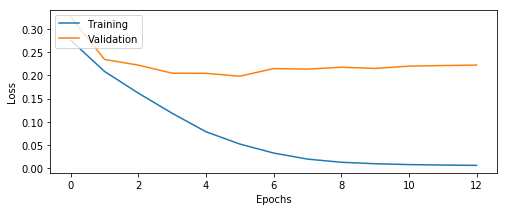
\includegraphics[width=\linewidth]{val_loss}
		\caption{Loss}
		\label{fig:hista}
	\end{subfigure}
	\hspace*{\fill} % separation between the subfigures
	\begin{subfigure}{0.49\textwidth}
		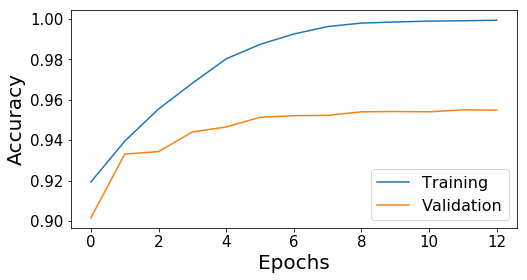
\includegraphics[width=\linewidth]{val_acc}
		\caption{Accuracy}
		\label{fig:histb}
	\end{subfigure}
	\caption{Loss and accuracy of the final enlarged model during training on the reduced training set and the validation set.}
	\label{fig:val_graphs}
\end{figure}

%talk about the hyperparameters


\section*{Results}

The final model (called enlarged in Table \ref{tab:def-hyper}) has been trained on the entire training set and evaluated on the test set.

%show confusion matrix
%show worst predictions (high probability but wrong)
%more thorough search of hyperparameters may be needed

\end{document}




















